\documentclass[crop,tikz]{standalone}

\usetikzlibrary{angles,calc}
\tikzset{>=latex}

\begin{document}
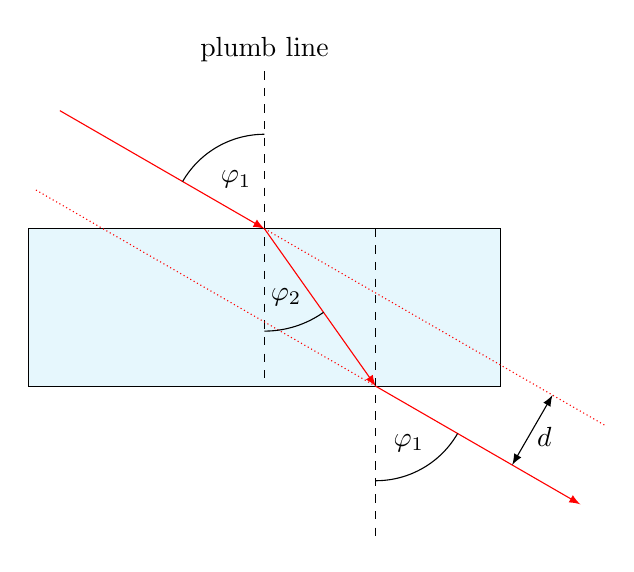
\begin{tikzpicture}
  \pgfmathsetmacro{\Width}{6};
  \pgfmathsetmacro{\Height}{2};
  \pgfmathsetmacro{\RefractionindexA}{1};
  \pgfmathsetmacro{\RefractionindexB}{1.5};
  \pgfmathsetmacro{\AngleA}{60};
  \pgfmathsetmacro{\AngleB}{asin(\RefractionindexA*sin(\AngleA)/\RefractionindexB)};
  \pgfmathsetmacro{\ParallelDistance}{\Height*sin(\AngleA-\AngleB)/cos(\AngleB)};
  % 
  \draw[fill=cyan!10] ({-\Width/2},0) rectangle ({\Width/2},{-\Height});
  \coordinate (O) at (0,0);
  \draw[dashed] (0,{\Height}) coordinate (LA) node[above] {plumb line} -- ++ (0,{-2*\Height}) coordinate (LD);
  \draw[->,red] ({90+\AngleA}:{\Width/2}) coordinate (A) -- (O);
  \draw[->,red] (O) -- ({-90+\AngleB}:{\Height/cos(\AngleB)}) coordinate (B);
  \draw[dashed] (B)++(0,{\Height}) coordinate (LB) -- ++(0,{-2*\Height}) coordinate (LC);
  \draw[->,red] (B) -- ++({-90+\AngleA}:{\Width/2}) coordinate (C);
  \draw[densely dotted,red] (B) -- ++ ({90+\AngleA}:5) coordinate (P);
  \draw[densely dotted,red] (O) -- ++ ({-90+\AngleA}:5);
  % 
  \draw[<->] (B)++({-90+\AngleA}:{\Width/3}) coordinate (D1) -- ++({\AngleA}:{\ParallelDistance}) coordinate (D2)node at ($(D1)!0.5!(D2)!-0.5em!90:(D2)$) {$d$};
  % 
  \pic[draw,angle radius=1.2cm,pic text={$\varphi_1$},angle eccentricity=0.6] {angle = LA--O--A};
  \pic[draw,angle radius=1.3cm,pic text={$\varphi_2$},angle eccentricity=0.7] {angle = LD--O--B};
  \pic[draw,angle radius=1.2cm,pic text={$\varphi_1$},angle eccentricity=0.7] {angle = LC--B--C};
\end{tikzpicture}
\end{document}
